\subsection{Batasan Implementasi}

Batasan-batasan yang diterapkan pada implementasi prototipe integrasi DecMed-PGHD ditetapkan sebagai berikut,

\begin{enumerate}
    \item Aplikasi PGHD pasien diimplementasikan sebagai aplikasi Android.
    Pengujian integrasi PGHD dilakukan pada satu perangkat Android dan satu komputer sebagai server, dan memakai \textit{smart band} untuk mensimulasikan pengambilan data dari \textit{wearable}.
    \item Data PGHD otomatis diperoleh melalui Health Connect (API kesehatan bawaan Android) dan sensor perangkat Android.
    Data dari wearable pada pengujian berasal dari Mi Smart Band 9 Active yang disinkronkan ke Health Connect melalui aplikasi Mi Fitness.
    \item Data yang berasal dari sensor perangkat Android dikonversi menjadi tipe data kesehatan yang lebih mudah dipahami pengguna, seperti langkah, aktivitas, jarak, dan tipe pengukuran lain yang didukung oleh implementasi.
    \item Data PGHD disimpan secara lokal pada perangkat pasien sebelum dibentuk menjadi \textit{batch} dan dikirim.
    Penyimpanan lokal pada prototipe ini tidak menerapkan enkripsi basis data lokal.
    \item IPFS, IOTA dan IOTA Gas Station yang digunakan berada pada server dan diakses dari komputer pengembangan melalui SSH \textit{tunneling}.
    \item \textit{Smart contract} yang digunakan merupakan paket Move DecMed yang telah diperluas dengan mekanisme PGHD\@.
    \item Pengujian dilakukan untuk skenario satu pasien, satu perangkat Android, satu perangkat \textit{wearable}, satu buah server PRE, dan satu \textit{client} tenaga kesehatan yang dijalankan dari komputer pengembangan.
\end{enumerate}

\subsection{Kakas dan Lingkungan yang Digunakan}

Implementasi DecMed-PGHD dilakukan pada lingkungan komputer lokal dengan dukungan layanan eksternal berupa jaringan IOTA, IPFS, dan IOTA Gas Station yang dijalankan pada server lokal.
Kakas yang digunakan terdiri atas perangkat keras, bahasa pemrograman, \textit{framework client}, \textit{framework backend}, kakas Android, kakas \textit{blockchain}, dan kakas \textit{containerization}.
Ringkasan kakas dan teknologi yang digunakan dapat dilihat pada Tabel~\ref{tab:kakas-implementasi-decmed-pghd} pada Lampiran~\ref{app:kakas-implementasi-decmed-pghd}.

Secara umum, implementasi dibagi ke dalam beberapa komponen.
\textit{\textit{Client} } Android pasien dibangun menggunakan Kotlin, Jetpack Compose, Health Connect, Room, WorkManager, dan \textit{shared library} Rust melalui JNI\@.
\textit{\textit{Client} ministry} dan \textit{client} tenaga kesehatan dibangun menggunakan Tauri, SvelteKit, TypeScript, dan Rust dengan mengutilisasi \textit{client} DecMed lama yang diperluas fungsinya untuk PGHD\@.
Komponen PRE dibangun menggunakan Rust dengan \textit{framework} Axum, Redis sebagai penyimpanan material akses sementara, IPFS sebagai penyimpanan \textit{payload} terenkripsi, dan jaringan IOTA pada server sebagai penyimpanan metadata serta mekanisme akses berbasis \textit{smart contract} Move.
% Arsitektur implementasi dapat dilihat pada Gambar~\ref{fig:arsitektur-implementasi}.

% \begin{figure}[htbp]
%     \centering
% 	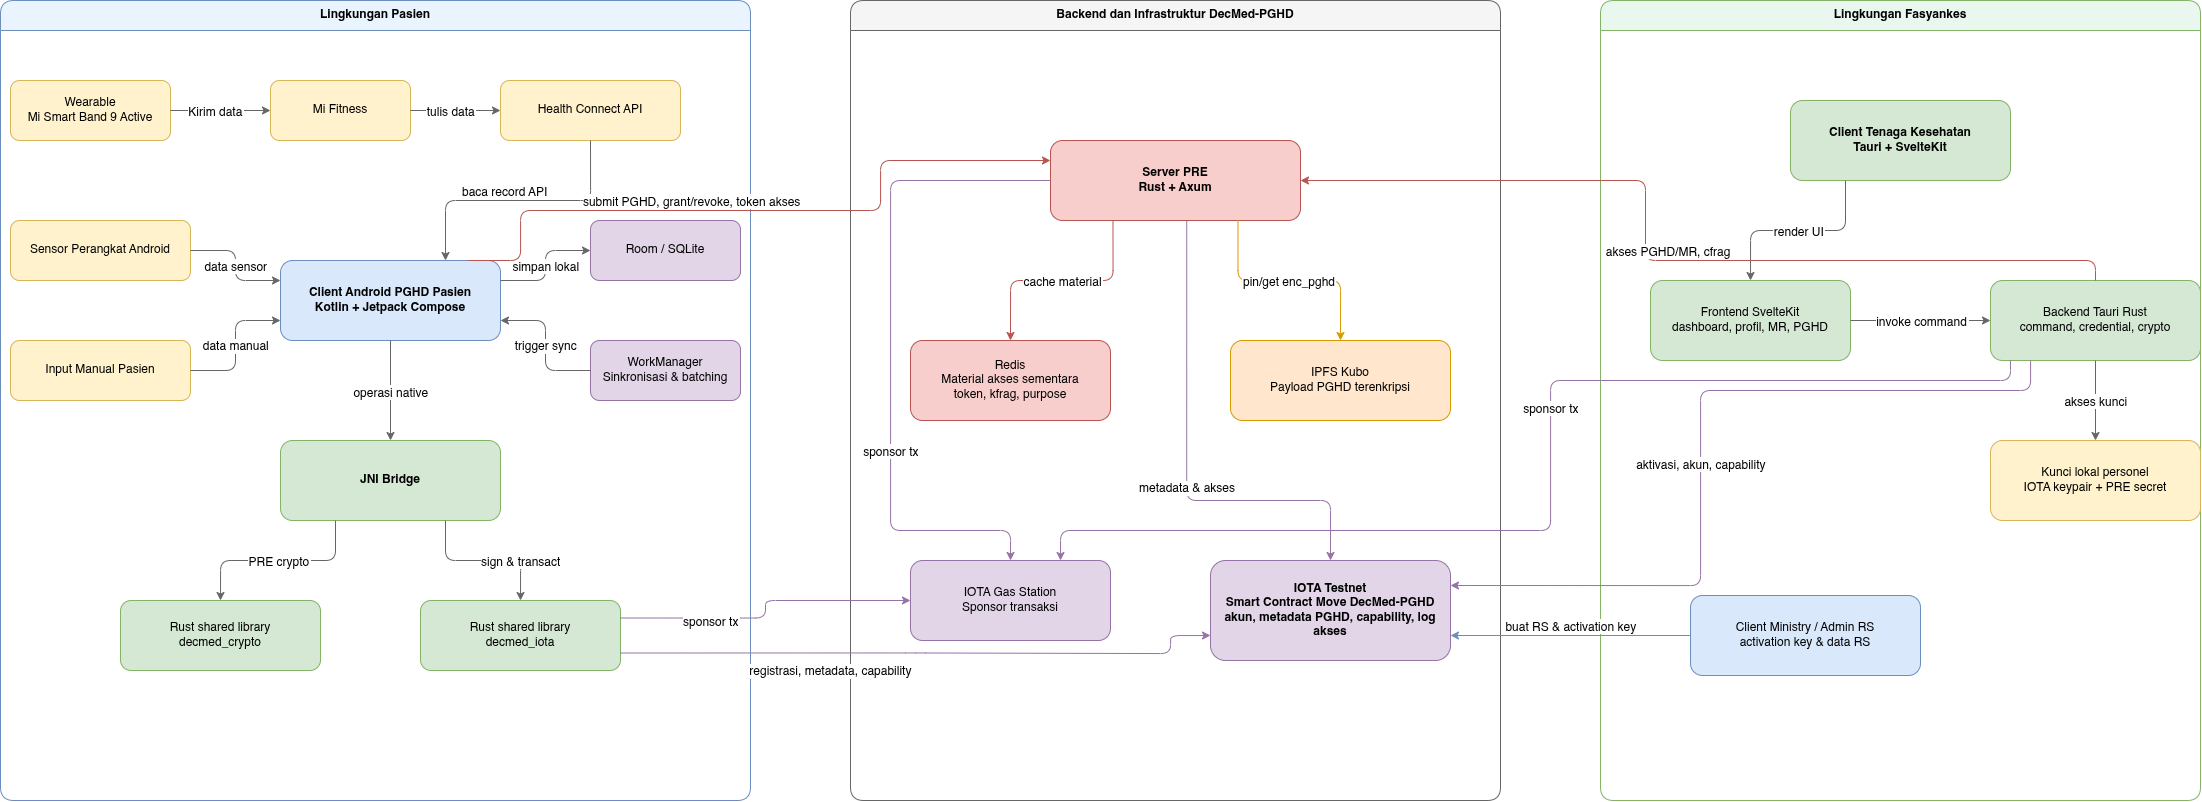
\includegraphics[width=\textwidth]{resources/chapter-4/Arsitektur Implementasi.png}
% 	\caption{Arsitektur Implementasi Sistem DecMed-PGHD}\label{fig:arsitektur-implementasi}
% \end{figure}


JNI (\textit{Java Native Interface}) adalah mekanisme interoperabilitas yang memungkinkan kode pada lingkungan Java/Kotlin memanggil fungsi \textit{native} yang dikompilasi ke \textit{shared library}.
Pada \textit{client} Android PGHD, JNI digunakan untuk menghubungkan kode Kotlin dengan dua \textit{shared library} Rust, yaitu \texttt{decmed\_crypto} dan \texttt{decmed\_iota}.
Penggunaan JNI dilakukan untuk mengurangi kebutuhan penulisan ulang kode DecMed ke Kotlin.
Pada sisi kriptografi (\texttt{decmed\_crypto}), modul ini dibuat karena mekanisme \textit{proxy re-encryption} yang digunakan oleh PGHD membutuhkan objek Umbral PRE seperti \textit{capsule}, \textit{key fragment}, dan \textit{capsule fragment}.
Jika seluruh fitur kriptografi ditulis secara \textit{native} pada Kotlin Android, maka implementasi tersebut tidak hanya memanggil \textit{primitive} kriptografi Android seperti AES-GCM, ECDH, atau ECDSA, tetapi harus membangun library Umbral PRE lengkap pada Android.
Hal ini terjadi karena Android/Kotlin tidak menyediakan implementasi bawaan untuk objek dan alur Umbral PRE yang digunakan oleh PRE dan \textit{client} pasien.
Oleh karena itu, \texttt{decmed\_crypto} tetap digunakan sebagai \textit{shared library} Rust agar \textit{client} Android memakai implementasi Umbral PRE yang sama dengan komponen DecMed lainnya.

Pada sisi IOTA, penggunaan \texttt{decmed\_iota} melalui JNI juga dipilih untuk menghindari penulisan ulang logika transaksi IOTA ke Kotlin.
Operasi yang dibutuhkan \textit{client} Android berisi pembentukan dan penandatanganan transaksi IOTA Move, termasuk serialisasi BCS, pembentukan \textit{programmable transaction block}, pemanggilan fungsi \textit{smart contract}, penggunaan \textit{shared object}, skema tanda tangan IOTA, serta integrasi dengan \textit{sponsored transaction}.
Kotlin memiliki SDK IOTA, namun implementasinya juga berupa \textit{binding} yang menggunakan JNI terhadap \textit{core} SDK Rust.
Dengan demikian, penggunaan \textit{shared library} Rust pada \texttt{decmed\_iota} mengikuti mekanisme yang sama, tetapi dibuat khusus untuk kebutuhan DecMed-PGHD sehingga fungsi yang diekspos ke Kotlin hanya fungsi yang diperlukan oleh aplikasi Android.

% Dengan menggunakan JNI, \textit{client} Android tetap dapat menggunakan API Android secara \textit{native} untuk UI, sensor, Health Connect, \textit{permission}, penyimpanan lokal, dan \textit{background worker}, sementara operasi kriptografi PRE dan transaksi IOTA tetap menggunakan implementasi Rust yang telah digunakan pada komponen DecMed lainnya.
% Pada implementasi ini, pemanggilan JNI dilakukan melalui kelas Kotlin \texttt{DecmedCryptoNative} dan \texttt{DecmedIotaNative}, sedangkan \textit{shared library} Rust dibangun untuk target Android dan dipaketkan ke dalam aplikasi melalui direktori \texttt{jniLibs}.
% Kelebihan dan kekurangan arsitektur menggunakan JNI dapat dilihat melalui Tabel~\ref{tab:plus-minus-jni-pghd}.

% \begin{styledxltabular}{|>{\raggedright\arraybackslash}p{0.22\textwidth}|>{\raggedright\arraybackslash}X|>{\raggedright\arraybackslash}X|}
%     \hiderowcolors
%     \caption{Kelebihan dan Kekurangan Penggunaan JNI pada \textit{\textit{Client} } Android PGHD}\label{tab:plus-minus-jni-pghd} \\
%     \hline
%     \rowcolor{headerBg}
%     \textbf{Aspek} & \textbf{Kelebihan} & \textbf{Kekurangan} \\
%     \hline
%     \showrowcolors
%     \endfirsthead
%     \hline
%     \rowcolor{headerBg}
%     \textbf{Aspek} & \textbf{Kelebihan} & \textbf{Kekurangan} \\
%     \hline
%     \endhead
%     \hline
%     \endfoot
%     \hline
%     \endlastfoot
%     Pengolahan dan Pengumpulan PGHD\@ & Akses sensor, Health Connect, \textit{permission}, dan UI tetap diimplementasikan secara \textit{native} Android sehingga sesuai dengan kebutuhan pengumpulan PGHD\@. & Logika yang membutuhkan akses langsung ke \textit{lifecycle} dan \textit{permission} Android tetap harus berada pada Kotlin, sehingga tidak seluruh komponen dapat dipindahkan ke Rust. \\
%     \hline
%     Kriptografi PGHD & Android dapat memakai implementasi Umbral PRE yang sama dengan PRE dan \textit{client} tenaga kesehatan tanpa membangun library Umbral PRE penuh pada Kotlin. & Diperlukan \textit{wrapper} JNI dan format data yang jelas antara Kotlin dan Rust untuk setiap operasi kriptografi. \\
%     \hline
%     Transaksi IOTA & Pembentukan dan penandatanganan transaksi IOTA Move dapat memakai implementasi Rust yang sesuai dengan ekosistem IOTA dan sudah digunakan oleh DecMed. & \textit{Shared library} Rust harus dibangun untuk target Android dan dipaketkan ke dalam aplikasi. \\
%     \hline
%     \textit{Development} & Mengurangi duplikasi implementasi protokol DecMed karena logika kriptografi dan IOTA tidak perlu ditulis ulang penuh pada Kotlin. & Perubahan antarmuka fungsi Rust perlu disinkronkan dengan \textit{wrapper} Kotlin agar pemanggilan JNI tetap sesuai. \\
%     \hline
%     \textit{Debugging} & \textit{Error} dari operasi kriptografi dan IOTA cukup dilihat pada modul Rust. & \textit{Debugging} lebih kompleks karena melibatkan Kotlin, batas pemanggilan JNI, dan kode Rust \textit{native}. \\
%     \hline
%     Performa & Cocok untuk operasi yang relatif berat seperti enkripsi, tanda tangan digital, derivasi kunci, dan transaksi IOTA\@. & Pemanggilan JNI memiliki \textit{overhead} sehingga tidak digunakan untuk pemrosesan setiap sampel sensor secara langsung. \\
%     \hline
% \end{styledxltabular}

\subsection{Konfigurasi Implementasi}

Terdapat beberapa konfigurasi yang harus dilakukan sebelum sistem DecMed-PGHD dapat dijalankan.
Konfigurasi tersebut meliputi konfigurasi jaringan IOTA, publikasi \textit{smart contract}, konfigurasi IOTA Gas Station, konfigurasi IPFS, konfigurasi PRE, konfigurasi \textit{client} desktop, dan konfigurasi pengembangan aplikasi Android.

\subsubsection{Konfigurasi Jaringan IOTA}

Implementasi DecMed-PGHD menggunakan jaringan IOTA yang dijalankan.
Jaringan ini digunakan untuk mempublikasikan \textit{smart contract} DecMed-PGHD, menyimpan metadata akun, menyimpan metadata PGHD, menyimpan \textit{capability} akses, dan mencatat status validasi data.

Konfigurasi \textit{client} IOTA dilakukan dengan memastikan IOTA CLI terhubung ke \textit{endpoint} RPC jaringan IOTA\@.
\textit{Endpoint} tersebut juga digunakan oleh PRE dan \textit{client} Android melalui variabel lingkungan \texttt{IOTA\_RPC\_URL}.
% Untuk melakukan konfigurasi \textit{environment smart contract}, konfigurasi yang dijalankan adalah sebagai berikut,

% \begin{lstlisting}[caption={Konfigurasi \textit{Endpoint} IOTA}, label={lst:konfigurasi-iota-server}, float=htb]
% ssh -N -L 127.0.0.1:9000:127.0.0.1:9000 user@103.107.4.64
% IOTA_RPC_URL=http://127.0.0.1:9000
% iota \textit{client} envs
% iota \textit{client} switch --env campus-localnet
% \end{lstlisting}

Apabila \textit{smart contract} dipublikasikan ulang, nilai \texttt{DECMED\_PACKAGE\_ID} dan \texttt{object ID} hasil publikasi harus diperbarui pada file konfigurasi PRE, \textit{client} Android, \textit{client ministry}, dan \textit{client} tenaga kesehatan.

\subsubsection{Konfigurasi IOTA Gas Station}

IOTA Gas Station digunakan agar transaksi yang dibuat oleh \textit{client} atau PRE dapat disponsori tanpa mengharuskan setiap \textit{client} memiliki saldo gas sendiri. 
Untuk mengkonfigurasi IOTA Gas Station, digunakan digunakan perintah \texttt{docker compose up} pada \textit{directory} tempat \textit{docker-compose file} berada.

Contoh konfigurasi \textit{endpoint} yang digunakan oleh \textit{client} adalah sebagai berikut,

\begin{lstlisting}[caption={Konfigurasi \textit{Endpoint} IOTA Gas Station}, label={lst:konfigurasi-gas-station}, float=htb]
GAS_STATION_BASE_URL=http://127.0.0.1:9528/v1
GAS_STATION_TOKEN=token
IOTA_GAS_BUDGET=10000000
IOTA_GAS_RESERVE_SECONDS=10
\end{lstlisting}

% Pada aplikasi Android, alamat \texttt{127.0.0.1} tidak menunjuk ke komputer pengembangan, melainkan ke perangkat Android itu sendiri. Oleh karena itu, endpoint Gas Station yang digunakan pada Android disesuaikan menjadi alamat IP komputer pada jaringan lokal, misalnya \texttt{http://192.168.1.10:9528/v1}, atau alamat lain yang dapat dijangkau oleh perangkat Android.

\subsubsection{Konfigurasi IPFS}

\textit{Payload} PGHD terenkripsi disimpan pada IPFS\@. 
Konfigurasi dari kluster IPFS didefinisikan dalam suatu \textit{docker-compose file}. 
Untuk menjalankan kluster IPFS dengan konfigurasi yang telah dijelaskan, digunakan perintah \texttt{docker compose up} pada \textit{directory} tempat \textit{docker-compose file} berada.

% \begin{lstlisting}[caption={Konfigurasi endpoint IPFS pada PRE}, label={lst:konfigurasi-ipfs-pre}, float=htb]
% IPFS_API_URL=http://127.0.0.1:5001
% \end{lstlisting}

% Pada implementasi ini, IPFS digunakan sebagai penyimpanan \textit{payload} terenkripsi\@. 
% Metadata seperti hash, CID hasil penyimpanan disimpan pada \textit{on-chain}.

\subsubsection{Konfigurasi Proxy Re-encryption}

PRE berfungsi sebagai komponen \textit{backend} yang melakukan verifikasi \textit{signature} PGHD, penyimpanan \textit{payload} terenkripsi ke IPFS, pembuatan \texttt{cfrag} untuk proses \textit{re-encryption}, serta komunikasi dengan \textit{smart contract} IOTA\@. 
PRE dijalankan sebagai \textit{service} Rust berbasis Axum. 
PRE membutuhkan konfigurasi alamat IOTA, \textit{object} ID \textit{smart contract}, \textit{endpoint} IPFS, \textit{endpoint} Gas Station, serta Redis.

% Contoh konfigurasi PRE adalah sebagai berikut,

% \begin{lstlisting}[caption={Konfigurasi PRE}, label={lst:konfigurasi-pre}, float=htb]
% PRE_BASE_URL=http://127.0.0.1:4100
% IOTA_RPC_URL=http://127.0.0.1:9000
% GAS_STATION_BASE_URL=http://127.0.0.1:9528/v1
% IPFS_API_URL=http://127.0.0.1:5001
% REDIS_URL=redis://:password@127.0.0.1:6379
% DECMED_PACKAGE_ID=0x...
% GLOBAL_ADMIN_IOTA_ADDRESS=0x...
% GLOBAL_ADMIN_IOTA_KEY_PAIR=iotaprivkey1...
% \end{lstlisting}

Redis digunakan untuk menyimpan material akses sementara seperti token akses dan \textit{material re-encryption}. 
Untuk menjalankan Redis, digunakan Redis-server lokal dengan menjalankan perintah \texttt{redis-server}.
Lalu untuk menjalankan PRE di lokal, digunakan perintah untuk menjalankan Rust \textit{package} yaitu dengan \texttt{cargo run}.

\subsubsection{Konfigurasi \textit{Client} Android PGHD}

\textit{Client} Android PGHD dibangun menggunakan Gradle, Android SDK, Kotlin, Jetpack Compose, Room, WorkManager, Health Connect, dan \textit{shared library} Rust. 
Sebelum \textit{build} Android dilakukan, \textit{shared library} Rust untuk kriptografi dan integrasi IOTA dibangun untuk target Android dan diletakkan pada direktori \texttt{jniLibs}.

\begin{lstlisting}[caption={\textit{Build} \textit{Shared Library} Rust untuk Android}, label={lst:build-shared-library-android}, float=htb]
export ANDROID_NDK_HOME=$ANDROID_HOME/ndk/<versi-ndk>
./crypto/decmed-crypto/build-android.sh
./crypto/decmed-iota/build-android.sh
\end{lstlisting}

\textit{Client} Android membutuhkan konfigurasi \textit{endpoint} PRE, \textit{endpoint} IOTA, \textit{endpoint} Gas Station, \textit{package} ID \textit{smart contract}, \textit{object} ID \textit{smart contract}, dan parameter \textit{batching} PGHD\@.
Contoh parameter yang digunakan adalah sebagai berikut,

\begin{lstlisting}[caption={Konfigurasi \textit{client} Android PGHD}, label={lst:konfigurasi-android-pghd}, float=htb]
PRE_BASE_URL=http://192.168.1.10:4100
IOTA_RPC_URL=http://192.168.1.10:9000
GAS_STATION_BASE_URL=http://192.168.1.10:9528/v1
DECMED_PACKAGE_ID=0x...
PGHD_SENSOR_INTERVAL_SECONDS=60
PGHD_BATCH_INTERVAL_MINUTES=15
PGHD_HEALTH_CONNECT_SYNC_INTERVAL_MINUTES=3
PGHD_EARLY_TRIGGER_BYTES=10485760
\end{lstlisting}

Selain konfigurasi \textit{endpoint}, aplikasi Android juga membutuhkan izin Android untuk akses aktivitas fisik, sensor, serta izin Health Connect. 
Izin Health Connect digunakan untuk membaca data kesehatan dari aplikasi dan perangkat eksternal seperti Mi Fitness untuk berkomunikasi dengan \textit{wearable} yang telah tersinkronisasi dengan Health Connect. 
Health Connect menyediakan berbagai tipe data kesehatan, struktur data \textit{time-series} seperti sampel detak jantung, serta mekanisme izin yang harus diminta aplikasi sebelum membaca atau menulis data \parencite{android_hc_write}.

\subsubsection{Konfigurasi \textit{Client} \textit{Ministry} dan \textit{Client} Tenaga Kesehatan}

\textit{Client} \textit{ministry} dan \textit{client} tenaga kesehatan dijalankan sebagai aplikasi desktop berbasis Tauri. 
Konfigurasi kedua \textit{client} membutuhkan konfigurasi \textit{endpoint} PRE, \textit{endpoint} IOTA, \textit{endpoint} Gas Station, \textit{package} ID \textit{smart contract}, \textit{object} ID \textit{smart contract}, dan \textit{secret key} akun yang berwenang. 
Contoh konfigurasi \textit{client} desktop adalah sebagai berikut,

\begin{lstlisting}[caption={Konfigurasi \textit{client} desktop DecMed}, label={lst:konfigurasi-client-desktop}, float=htb]
IOTA_RPC_URL=http://127.0.0.1:9000
GAS_STATION_BASE_URL=http://127.0.0.1:9528/v1
DECMED_PACKAGE_ID=0x...
DECMED_MINISTRY_ADMIN_ADDRESS=0x...
DECMED_MINISTRY_ADMIN_SECRET_KEY=iotaprivkey1...
\end{lstlisting}

